\documentclass[12pt,a4paper,oneside,openany,oneauthor,masterthesis,deansoffice]{mfipl}

\usepackage{float}
\usepackage{graphicx}
\usepackage{clrscode}
\usepackage{latexsym}
\usepackage{amsmath}
\usepackage{booktabs}


\begin{document}

\section*{Zadanie 1 -- Filtry nieliniowe RGB}
\subsection*{(a) Filtr minimalny}

$c_2 = (128,128,0)$, $\|c_2\| \approx 181{,}02$.
\[
\boxed{c_k = c_2 = (128, 128, 0)}
\]

\subsection*{(b) Filtr maksymalny}

$c_4 = (250,200,200)$, $\|c_4\| \approx 377{,}49$.
\[
\boxed{c_k = c_4 = (250, 200, 200)}
\]

\subsection*{(c) Filtr medianowy}

$c_6 = (200,200,200)$ z wartością $\sum_j \|c_6 - c_j\|$.
\[
\boxed{c_k = c_6 = (200, 200, 200)}
\]

\section*{Zadanie 2 -- Filtry uśredniający, Gaussa i $k$-NN}

\begin{figure}[H]
\centering
\includegraphics[width=0.45\textwidth]{zad2/1_Oryginal.png}
\caption{Obraz oryginalny.}
\end{figure}

\begin{figure}[H]
\centering
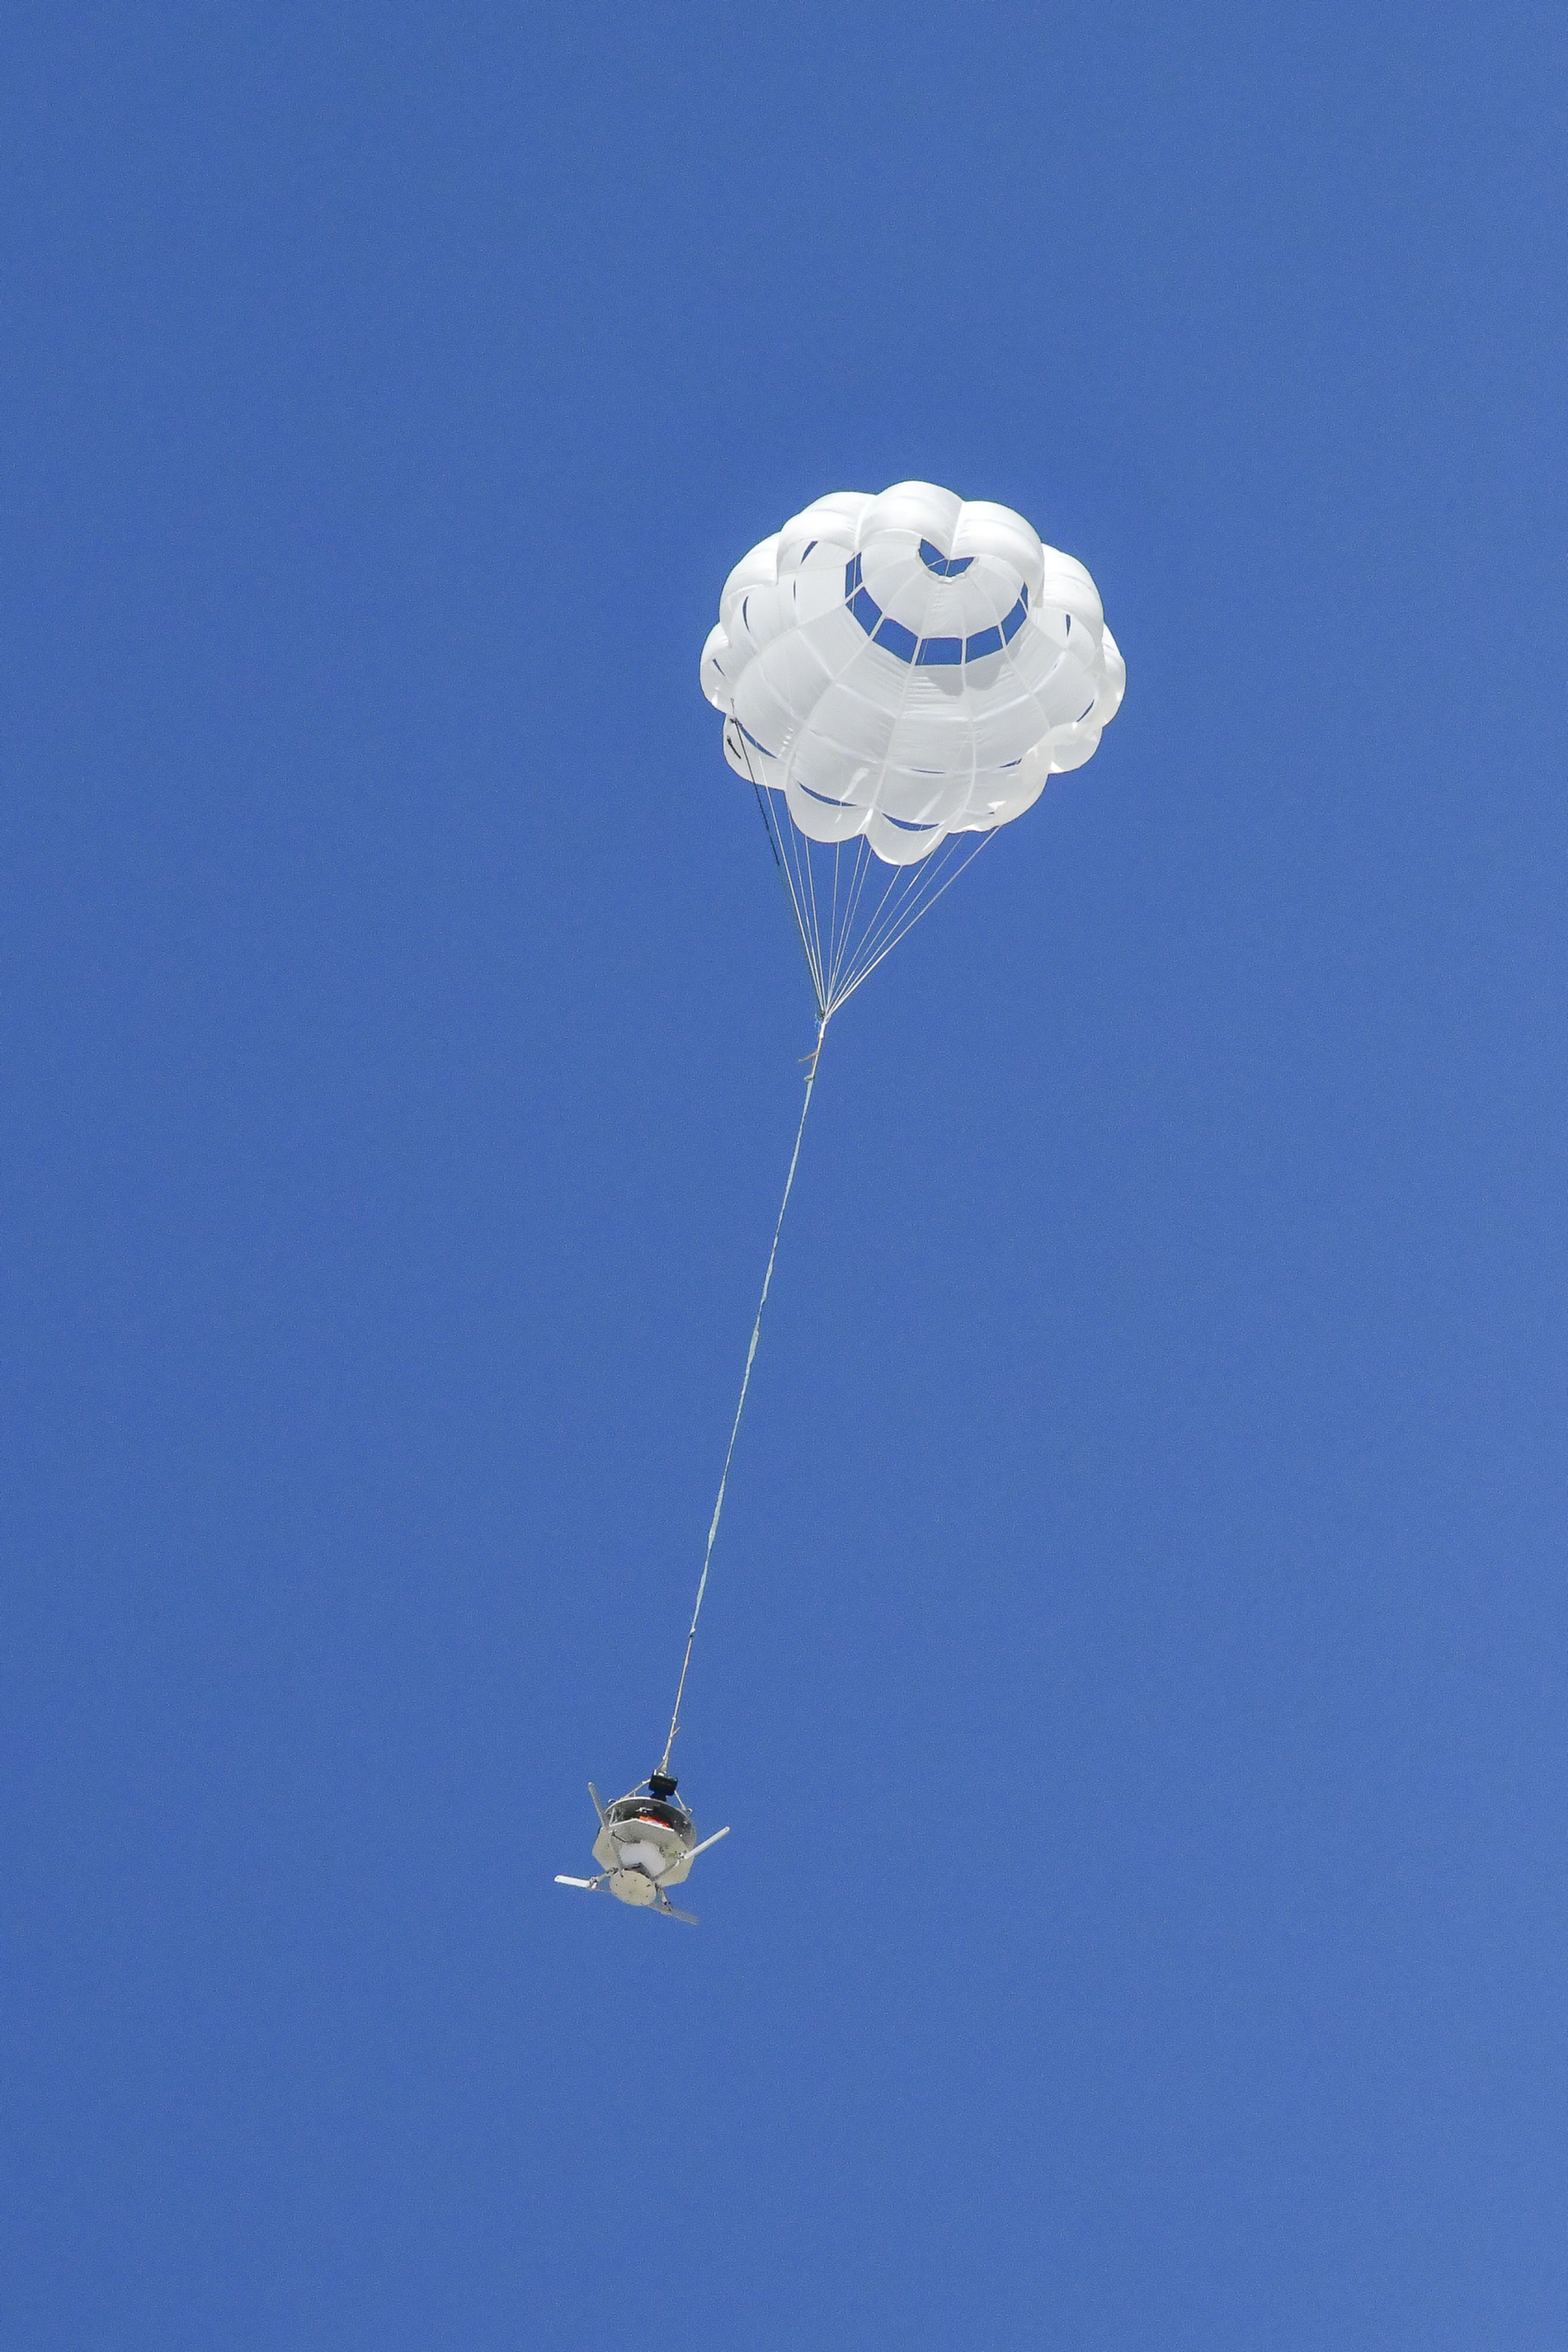
\includegraphics[width=0.45\textwidth]{zad2/2_Usredniajacy.png}
\caption{Filtr uśredniający $3\times 3$.}
\end{figure}

\begin{figure}[H]
\centering
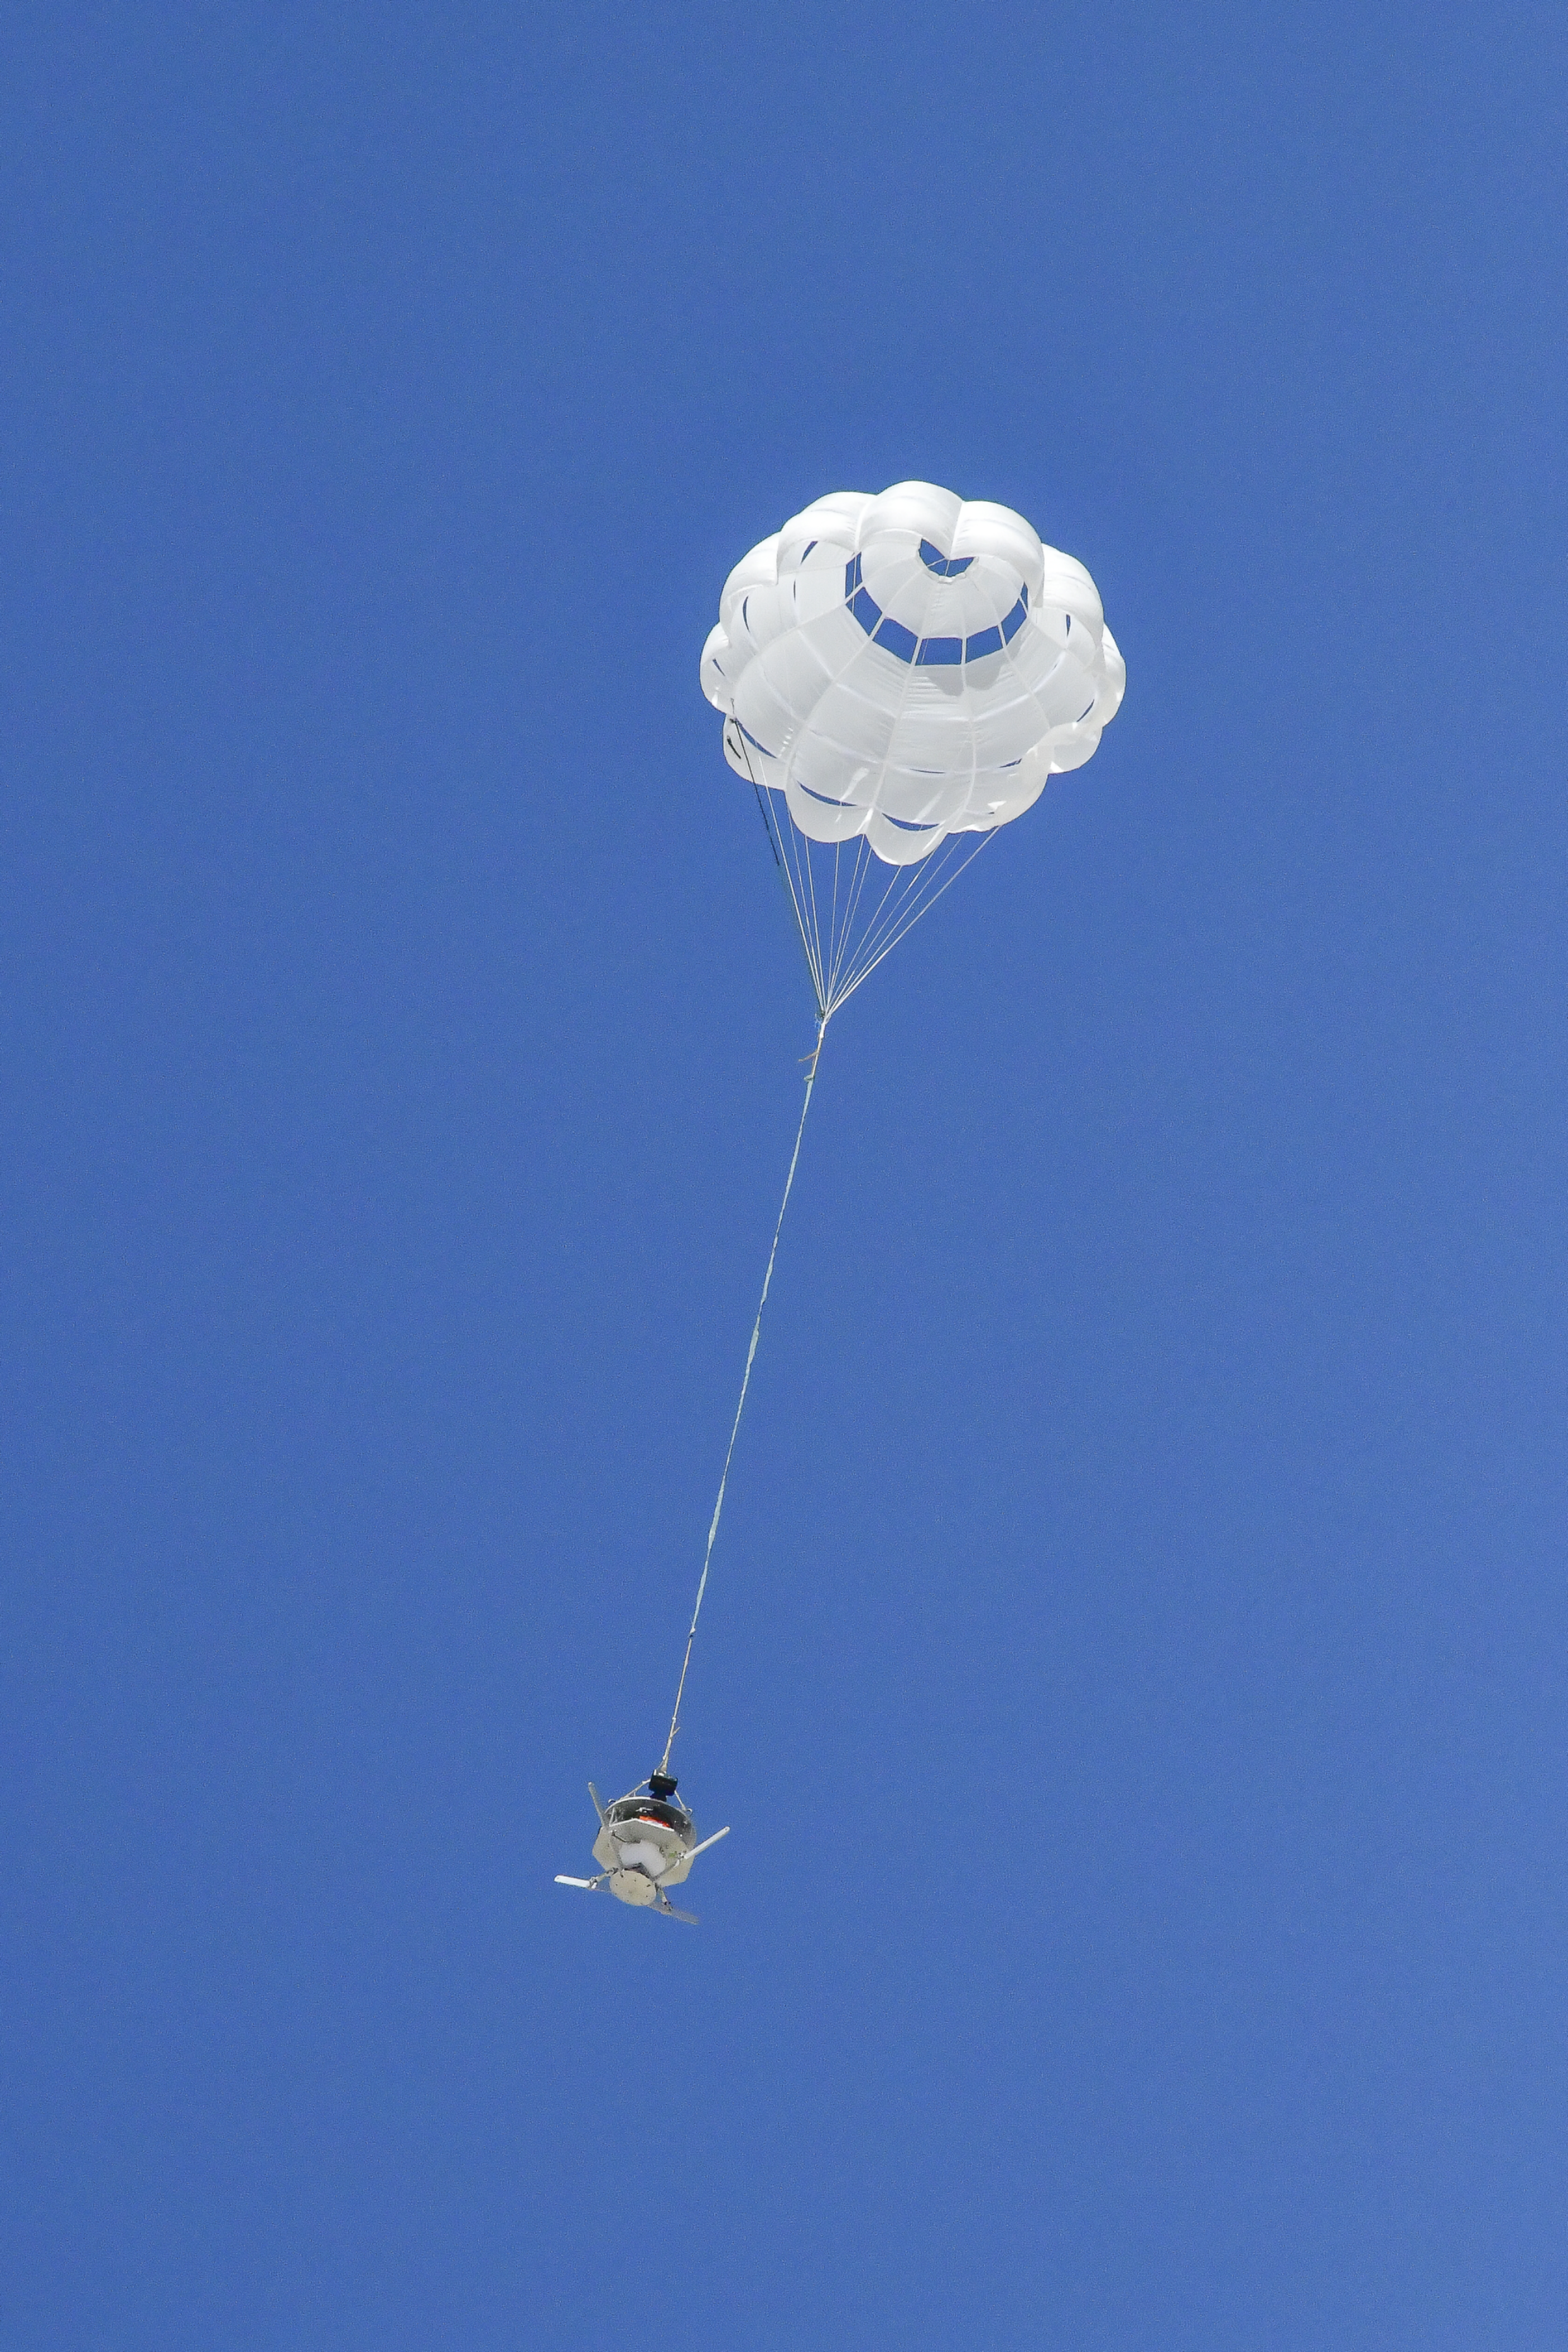
\includegraphics[width=0.45\textwidth]{zad2/3_Gauss.png}
\caption{Filtr Gaussa $3\times 3$ z $\sigma=2$.}
\end{figure}

\begin{figure}[H]
\centering
\includegraphics[width=0.45\textwidth]{zad2/4_kNN.png}
\caption{Filtr $k$-NN dla $k=6$ w oknie $3\times 3$.}
\end{figure}

\begin{figure}[H]
\centering
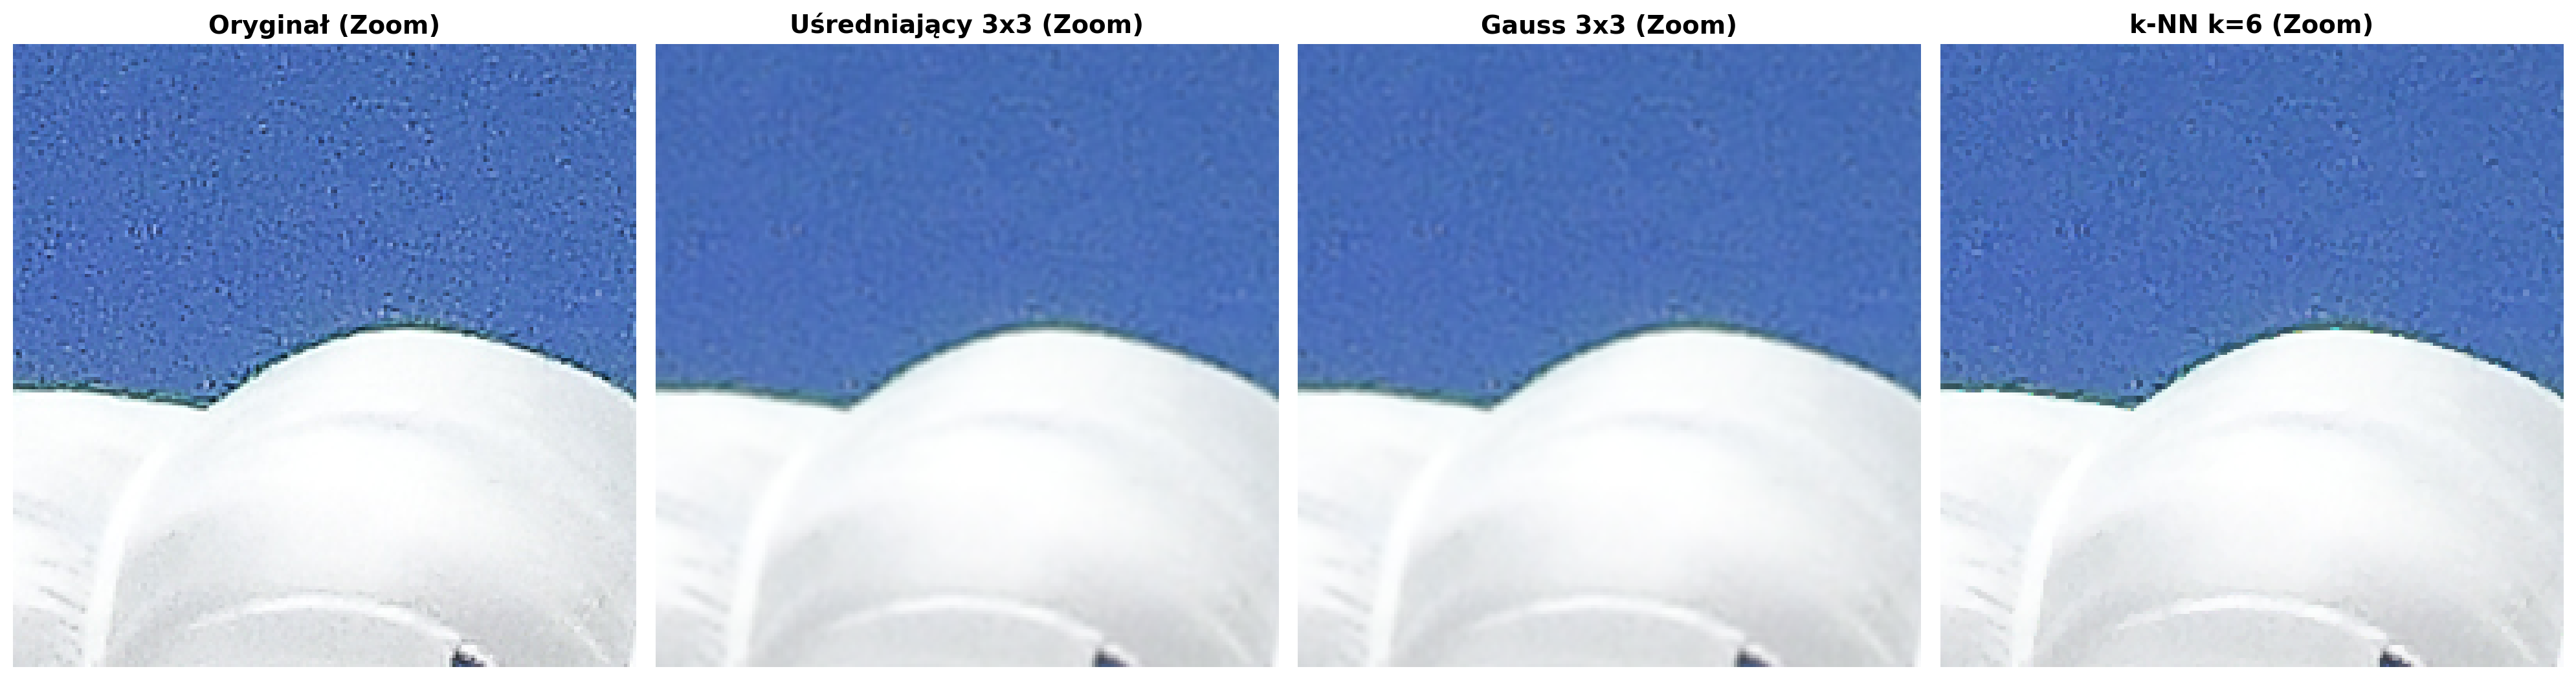
\includegraphics[width=\textwidth]{zad2/5_Zestawienie_Zoom.png}
\caption{Zestawienie powiększonego, najbardziej kontrastowego fragmentu obrazu dla każdej metody.}
\end{figure}

\subsection*{Charakterystyka wyników}

Filtr uśredniający i Gaussa silnie wygładzają obraz, ale rozmywają również krawędzie -- detale (np.\ litery, krawędzie spadochronu) tracą ostrość. Filtr $k$-NN jest filtrem zachowującym krawędzie: w każdym oknie wybiera $k$ wartości najbliższych pikselowi centralnemu, dzięki czemu skutecznie tłumi szum w obszarach jednorodnych, jednocześnie zachowując ostre przejścia między obszarami o różnym kolorze.

\section*{Zadanie 3 -- Filtry nieliniowe na obrazie \texttt{Jellyfish.png}}

\subsection*{(a) Eliminacja punktów izolowanych}

Filtr zastępuje piksel centralny średnią z otoczenia, jeżeli odległość euklidesowa pikselu centralnego od średniej $\mu$ otoczenia przekracza próg $\Theta = 25{,}5$ (ok. 10\% zakresu 8-bitowego).

\begin{figure}[H]
\centering
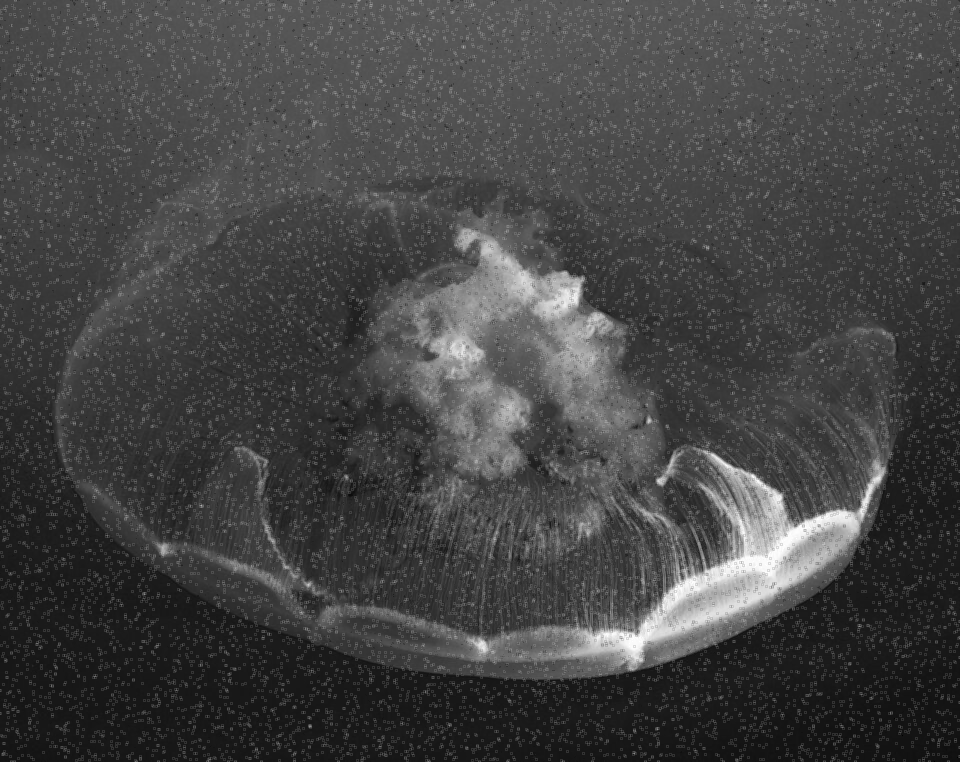
\includegraphics[width=0.45\textwidth]{zad3/a_Eliminacja_Izolowanych.png}
\caption{Filtr eliminacji punktów izolowanych ($\Theta \approx 10\%$).}
\end{figure}

\subsection*{(b) Filtr medianowy}

\begin{figure}[H]
\centering
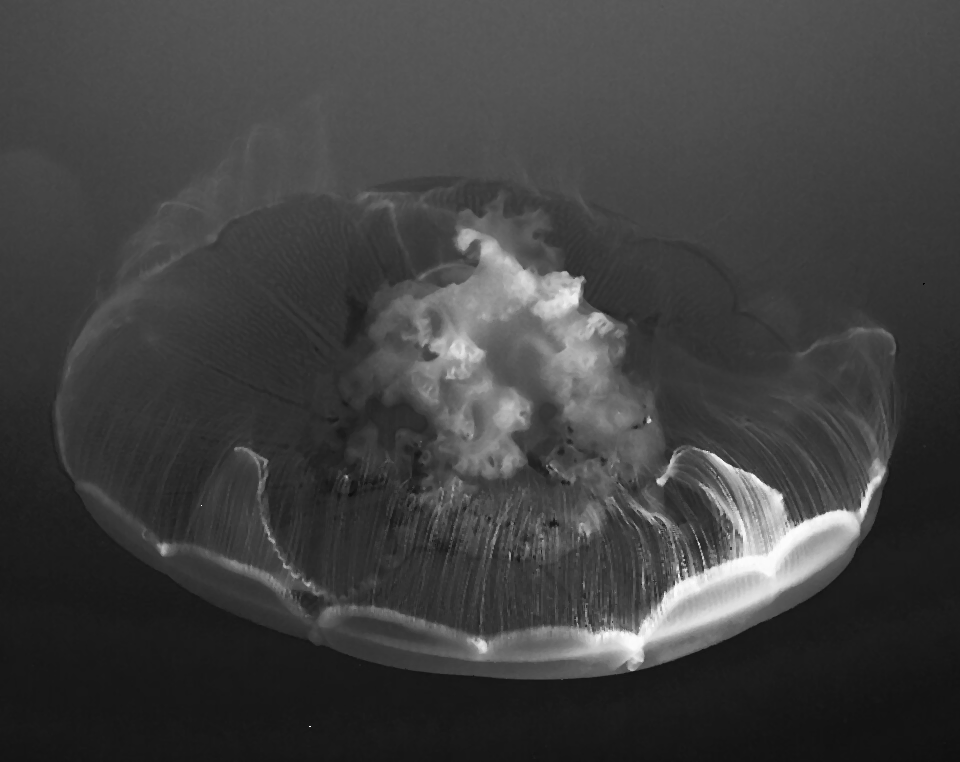
\includegraphics[width=0.45\textwidth]{zad3/b_Medianowy.png}
\caption{Filtr medianowy $3\times 3$.}
\end{figure}

\subsection*{(c) Filtr średniozakresowy (midrange)}

\begin{figure}[H]
\centering
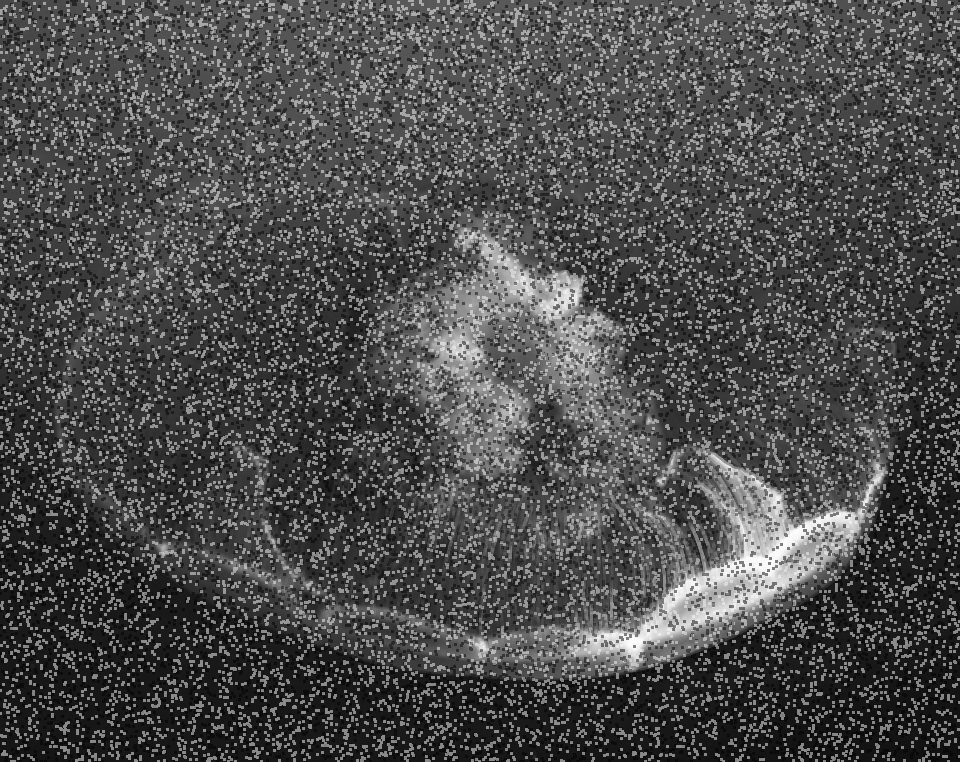
\includegraphics[width=0.45\textwidth]{zad3/c_Sredniozakresowy.png}
\caption{Filtr średniozakresowy.}
\end{figure}

\subsection*{(d) Filtr średniej uciętej (trimmed mean)}

Sortowane wartości okna z odrzuceniem $k=2$ skrajnych z każdej strony, średnia z pozostałych.

\begin{figure}[H]
\centering
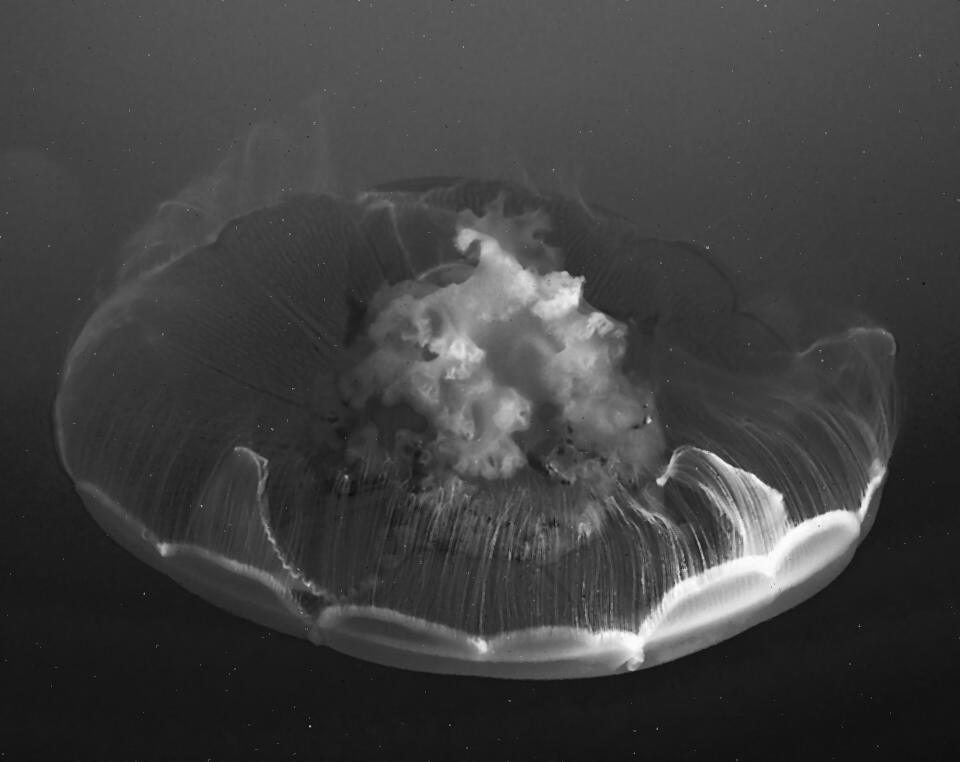
\includegraphics[width=0.45\textwidth]{zad3/d_Srednia_Ucieta.png}
\caption{Filtr średniej uciętej ($k=2$).}
\end{figure}

\subsection*{(e) Symmetric Nearest Neighbor}

Dla każdej z czterech par pikseli symetrycznych względem środka okna wybierany jest ten, który jest bliżej pikselowi centralnemu; wynik to średnia z czterech wybranych.

\begin{figure}[H]
\centering
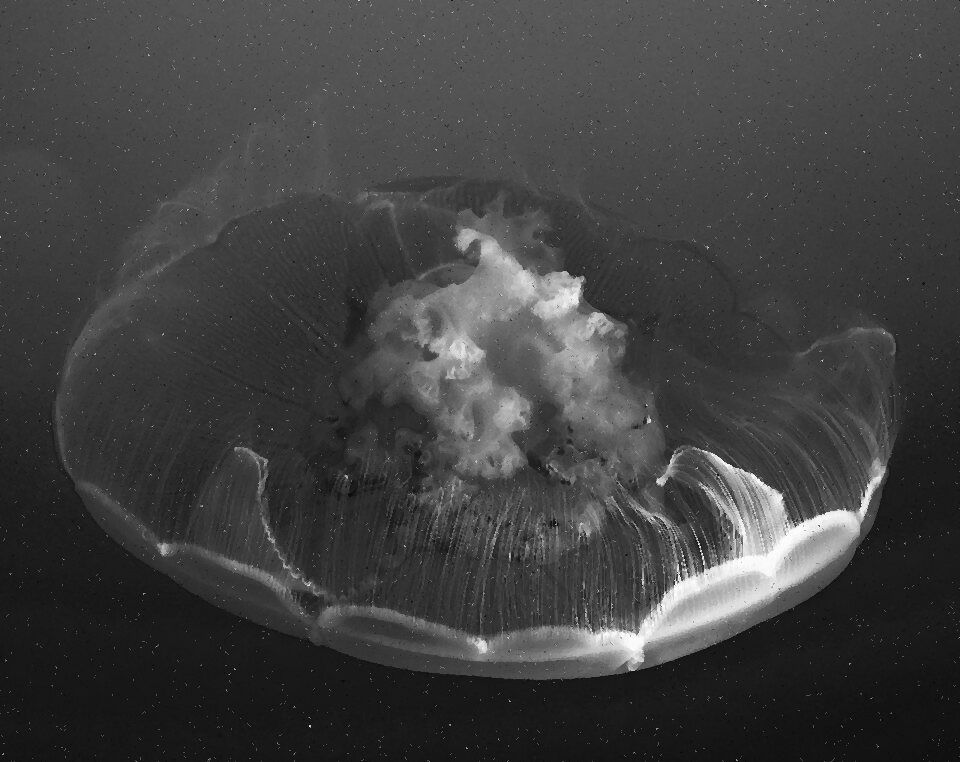
\includegraphics[width=0.45\textwidth]{zad3/e_Symmetric_NN.png}
\caption{Filtr Symmetric Nearest Neighbor (SNN).}
\end{figure}

\begin{figure}[H]
\centering
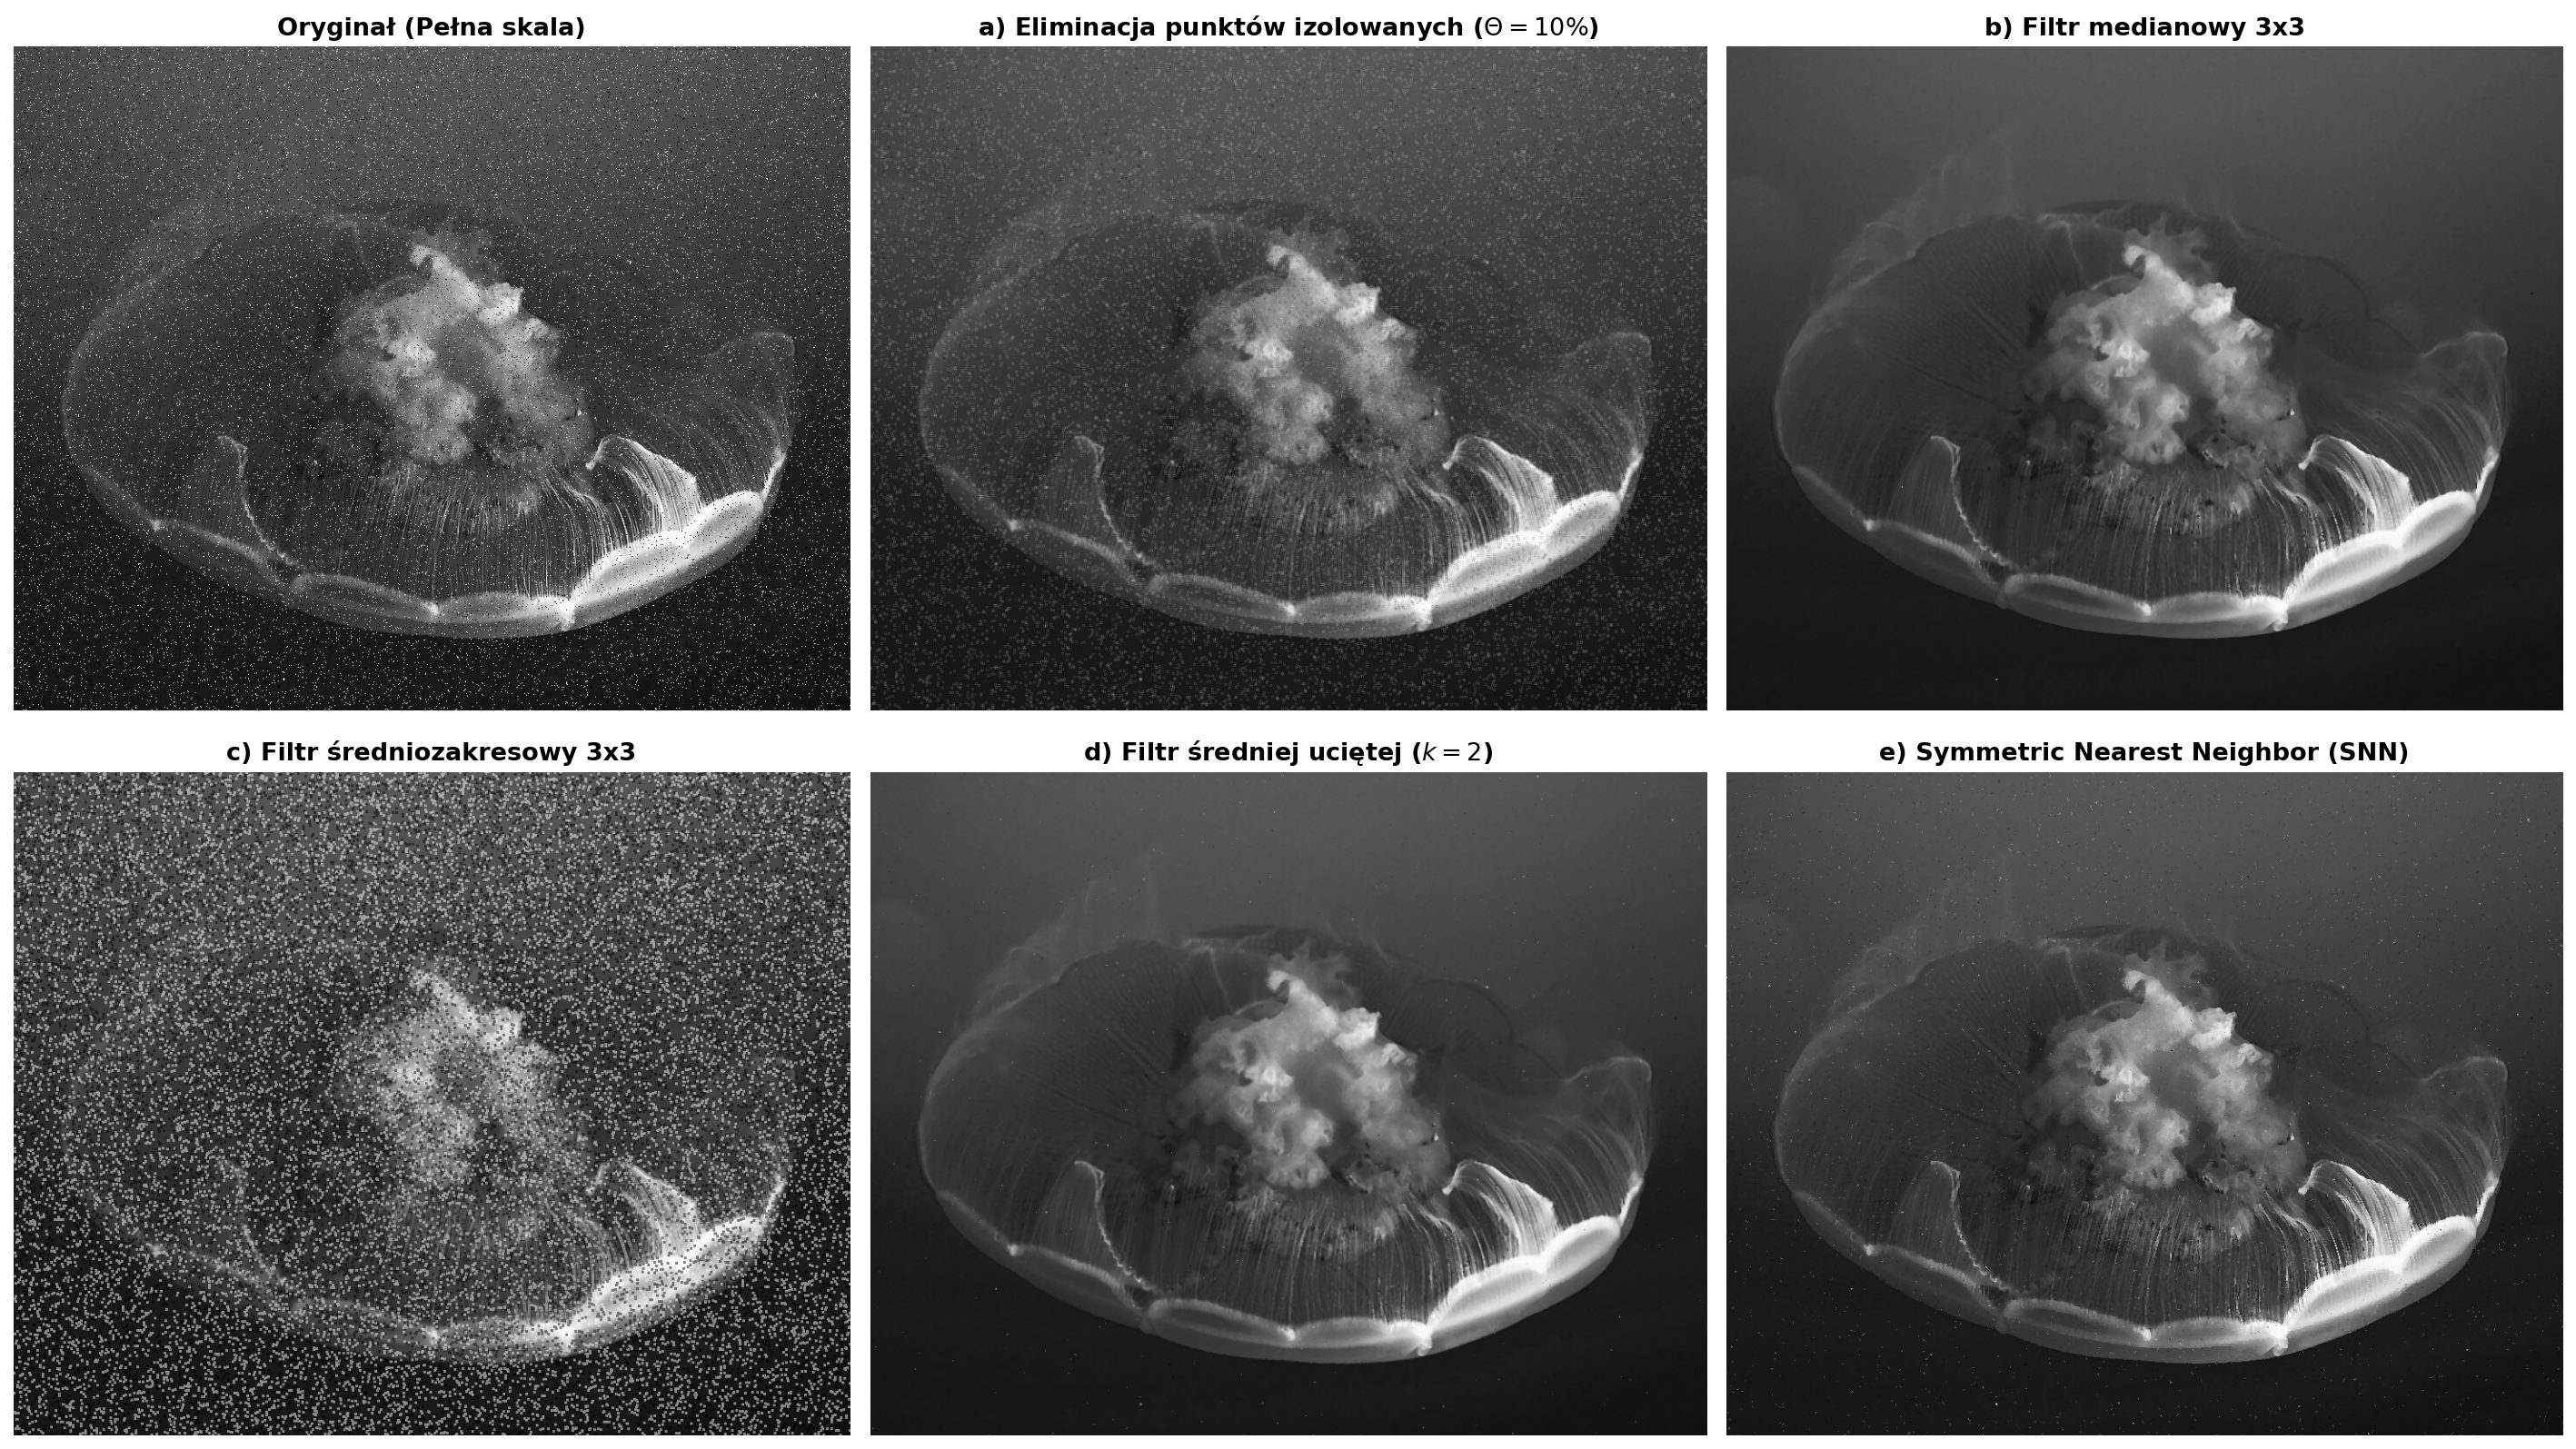
\includegraphics[width=\textwidth]{zad3/Zestawienie_Wynikowe_Pelne.png}
\caption{Zestawienie: oryginał oraz wyniki filtrów (a)--(e).}
\end{figure}

\subsection*{Charakterystyka filtrów}

Filtr (a) usuwa pojedyncze, izolowane piksele różniące się znacznie od otoczenia, pozostawiając resztę obrazu nietkniętą. Mediana (b) bardzo dobrze tłumi szum, jednocześnie zachowując krawędzie. Filtr średniozakresowy (c) jest najbardziej wrażliwy na szum (skrajne wartości dominują wynik). Średnia ucięta (d) jest kompromisem -- usuwa wartości skrajne i uśrednia resztę. SNN (e) najlepiej zachowuje krawędzie, ponieważ z każdej pary symetrycznej zawsze wybierany jest piksel bardziej zgodny z centrum, co utrudnia przeniknięcie wartości z drugiej strony krawędzi.

\section*{Zadanie 4 -- Korelacja, lokalizacja wzorca na obrazie}

\begin{figure}[H]
\centering
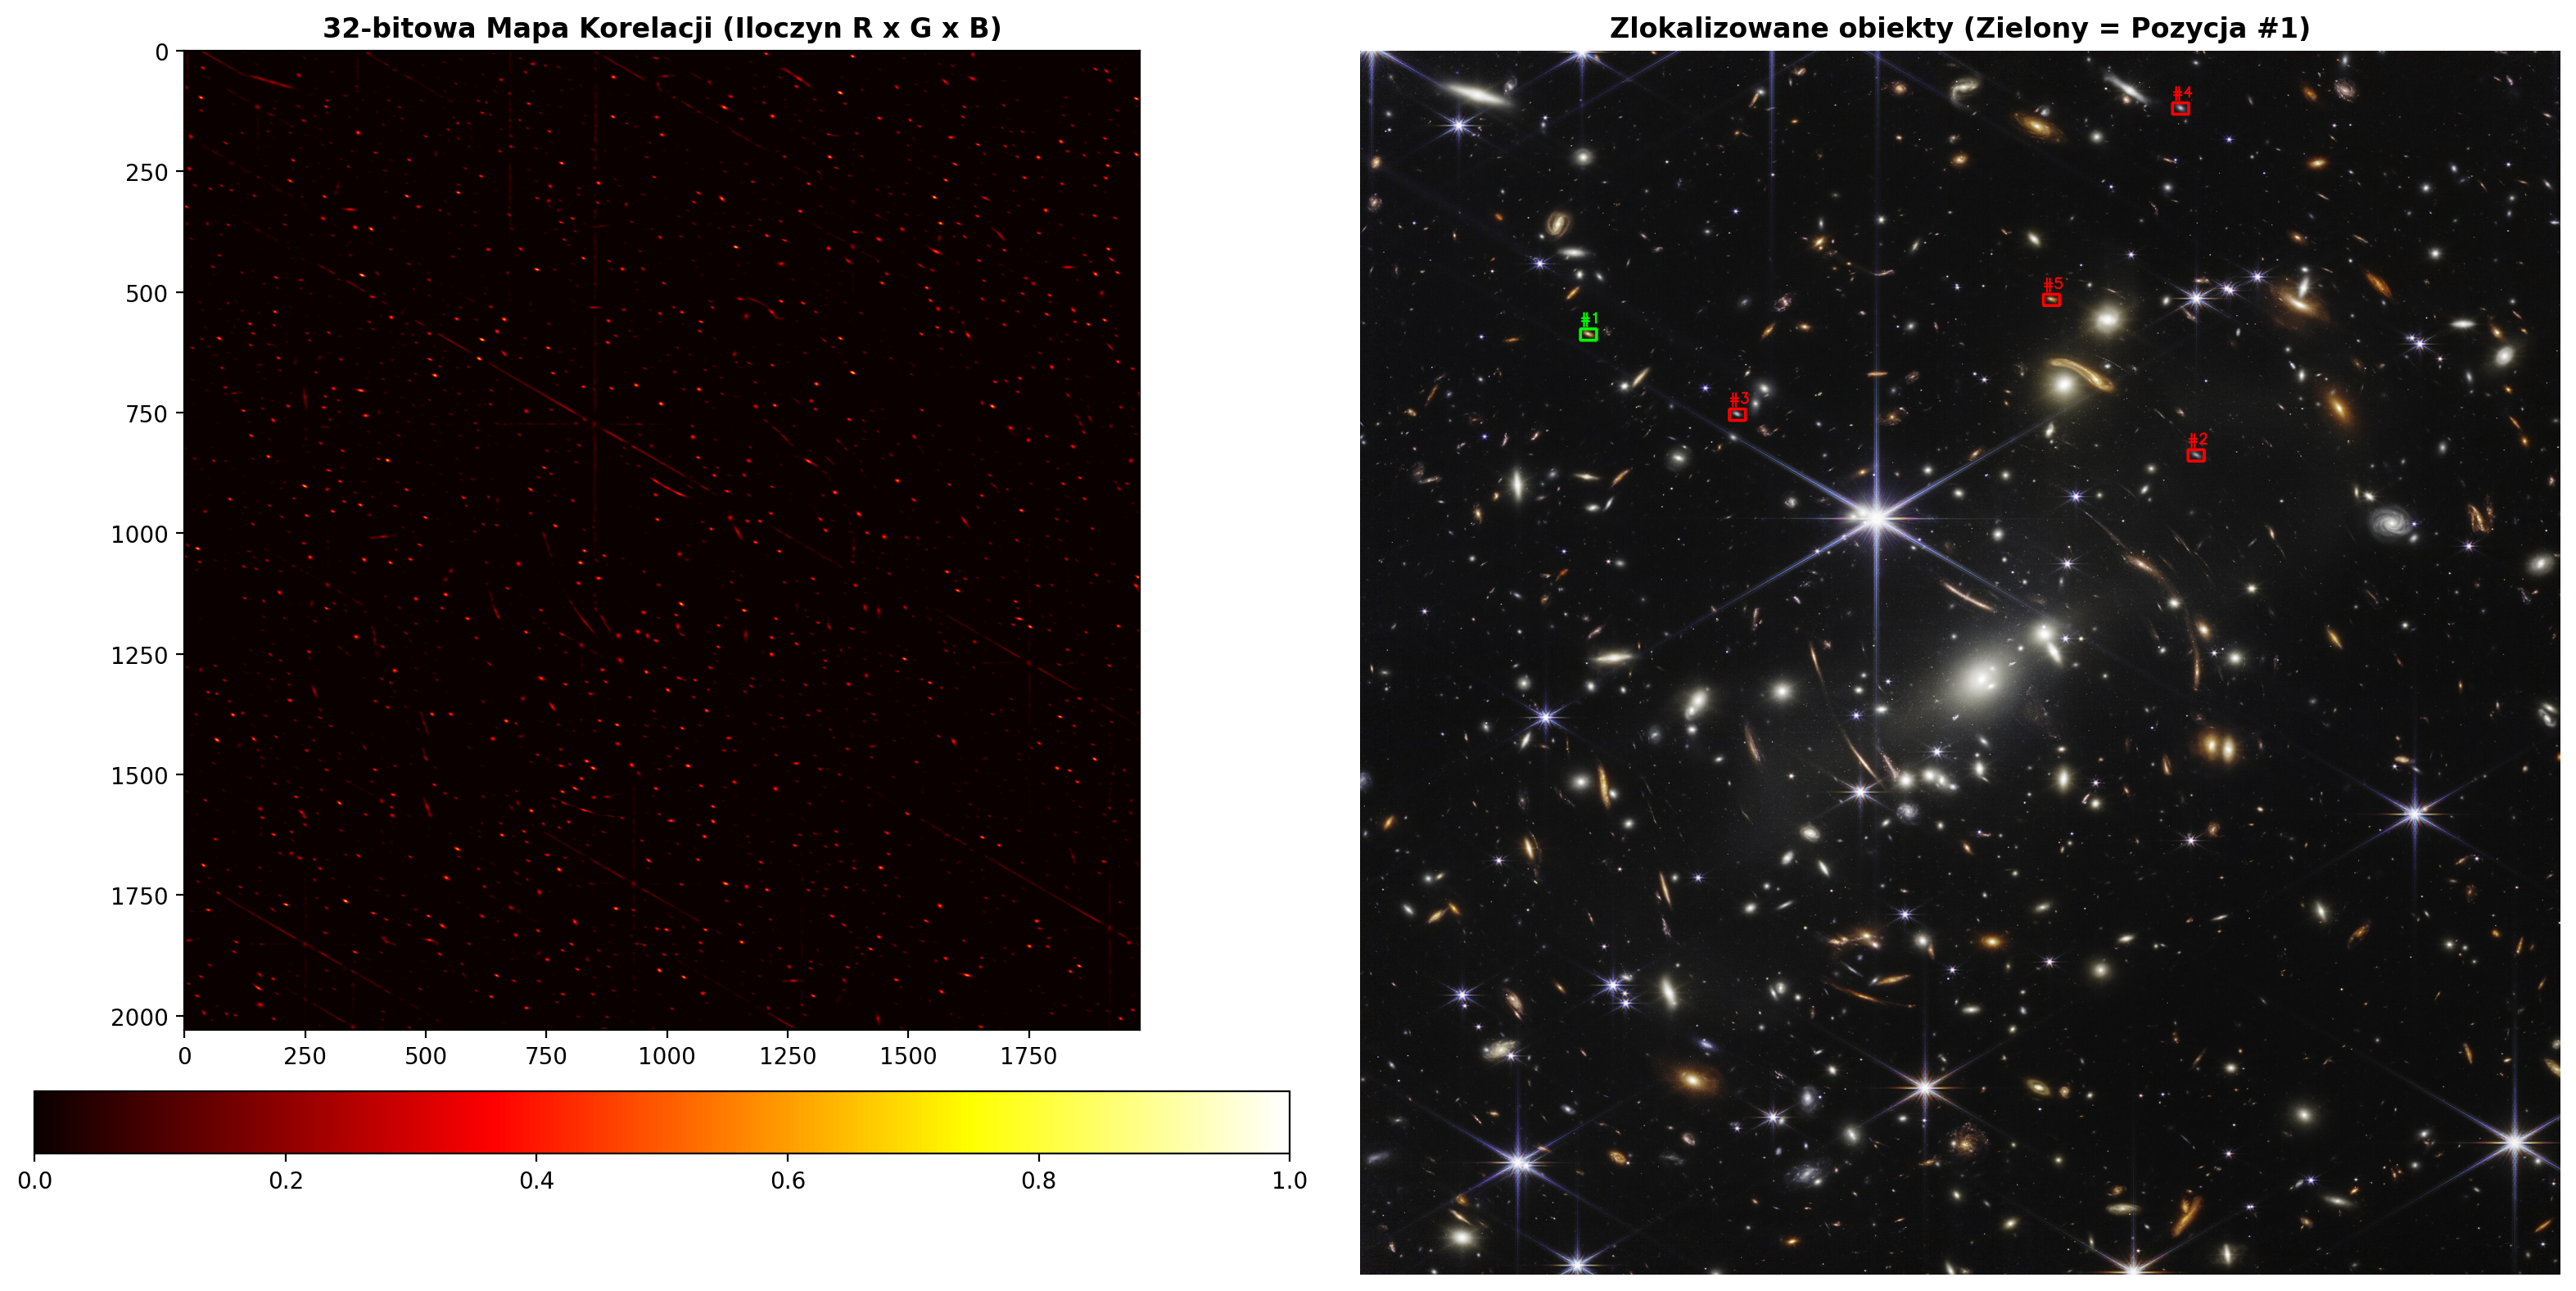
\includegraphics[width=\textwidth]{zad4/Zestawienie_Korelacji_Webb.png}
\caption{Zestawienie: 32-bitowa mapa korelacji (iloczyn $R \cdot G \cdot B$) oraz obraz z zaznaczonymi pięcioma najbardziej prawdopodobnymi pozycjami wzorca (zielona ramka -- pozycja \#1).}
\end{figure}

\begin{figure}[H]
\centering
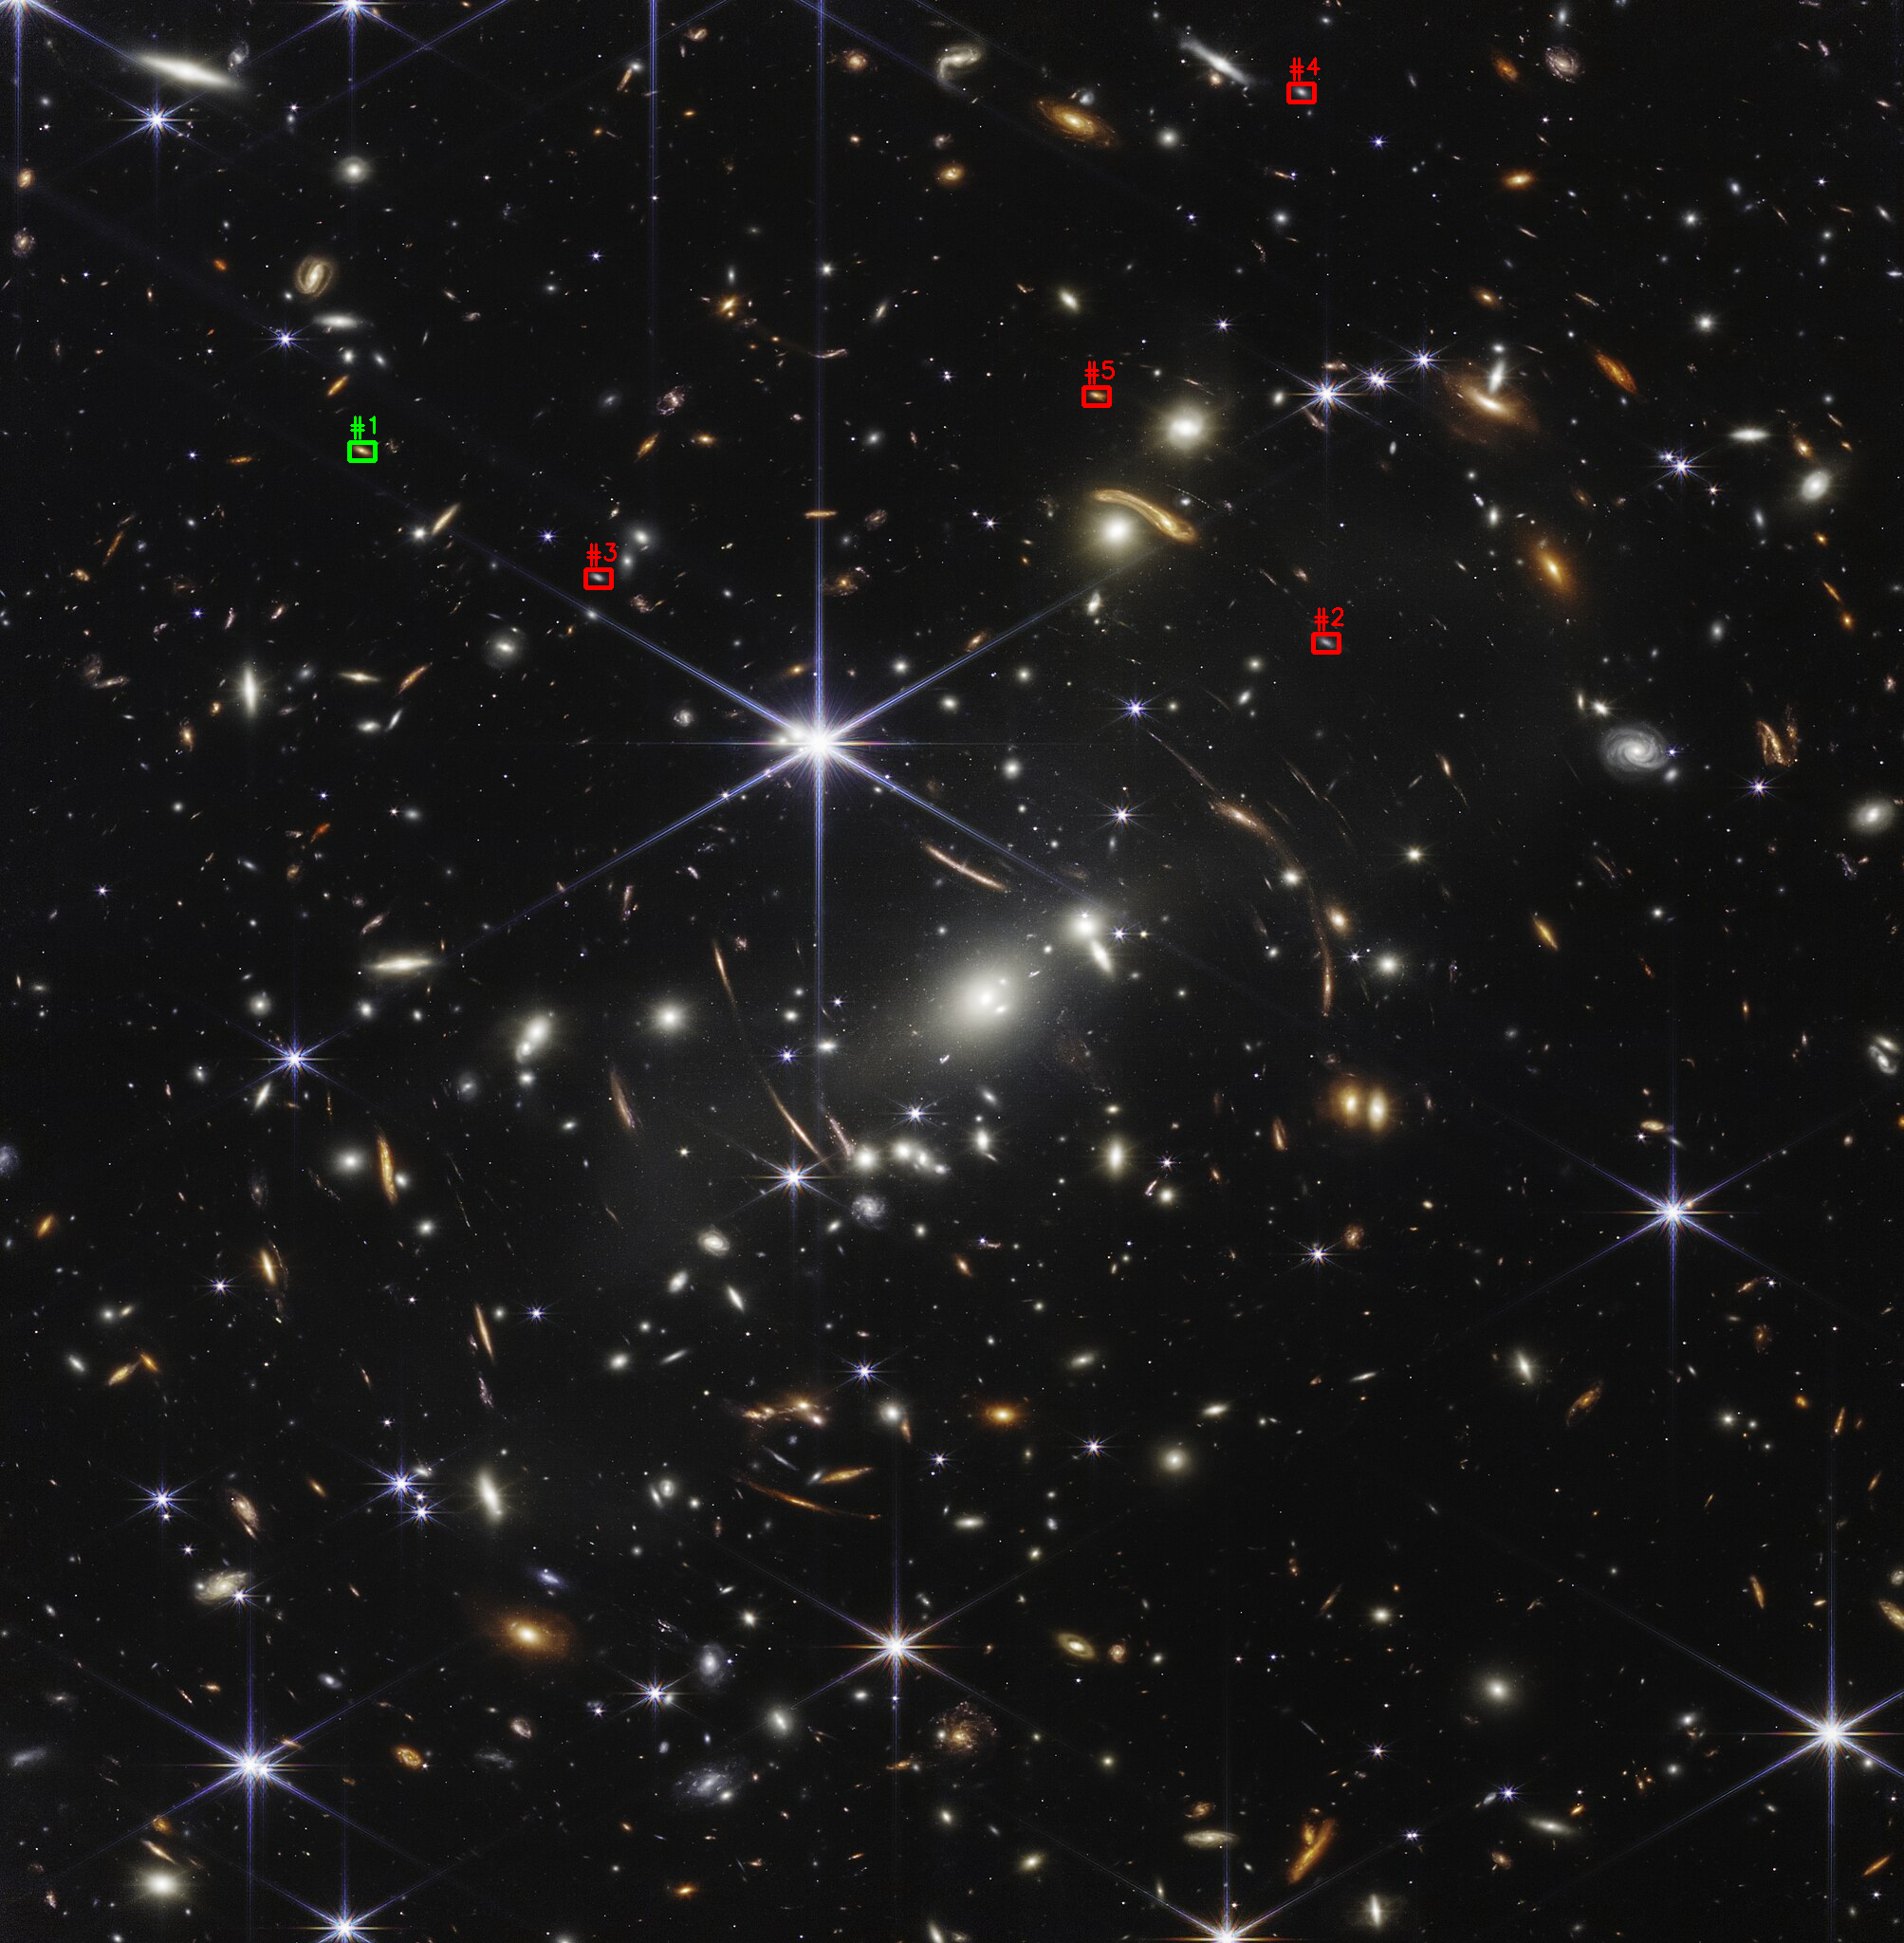
\includegraphics[width=0.7\textwidth]{zad4/Zlokalizowany_Wzorzec_Pelny.png}
\caption{Pełnowymiarowy obraz wynikowy z zaznaczonymi pięcioma kandydatami.}
\end{figure}

\section*{Zadanie 5 -- Korelacja, ocena zgodności sekcji ze wzorcem}

\subsection*{Zaproponowane kroki przetwarzania obrazu}

\paragraph{Krok 1: Lokalizacja wycinka za pomocą korelacji (Template Matching).}
Zanim porównamy obrazy, musimy wiedzieć, w którym dokładnie miejscu na dużym wzorcu znajduje się dany wycinek.

\paragraph{Krok 2: Obliczenie różnicy bezwzględnej (Absolute Difference).}
Obliczamy bezwzględną różnicę wartości pikseli pomiędzy wyciętym fragmentem wzorca ($W$) a badaną sekcją ($S$):

\paragraph{Krok 3: Progowanie (Binarizacja).}
Prosty próg (\emph{thresholding}). Ustawiamy wartość odcięcia na poziomie $30$ w skali $0$--$255$. Wszystkie piksele poniżej progu stają się całkowicie czarne, a powyżej -- całkowicie białe.

Otrzymujemy czysty, czarno-biały obraz (tzw.\ maskę błędów), na którym widoczne są wyłącznie rzeczywiste zmiany geometryczne.

\begin{figure}[H]
\centering
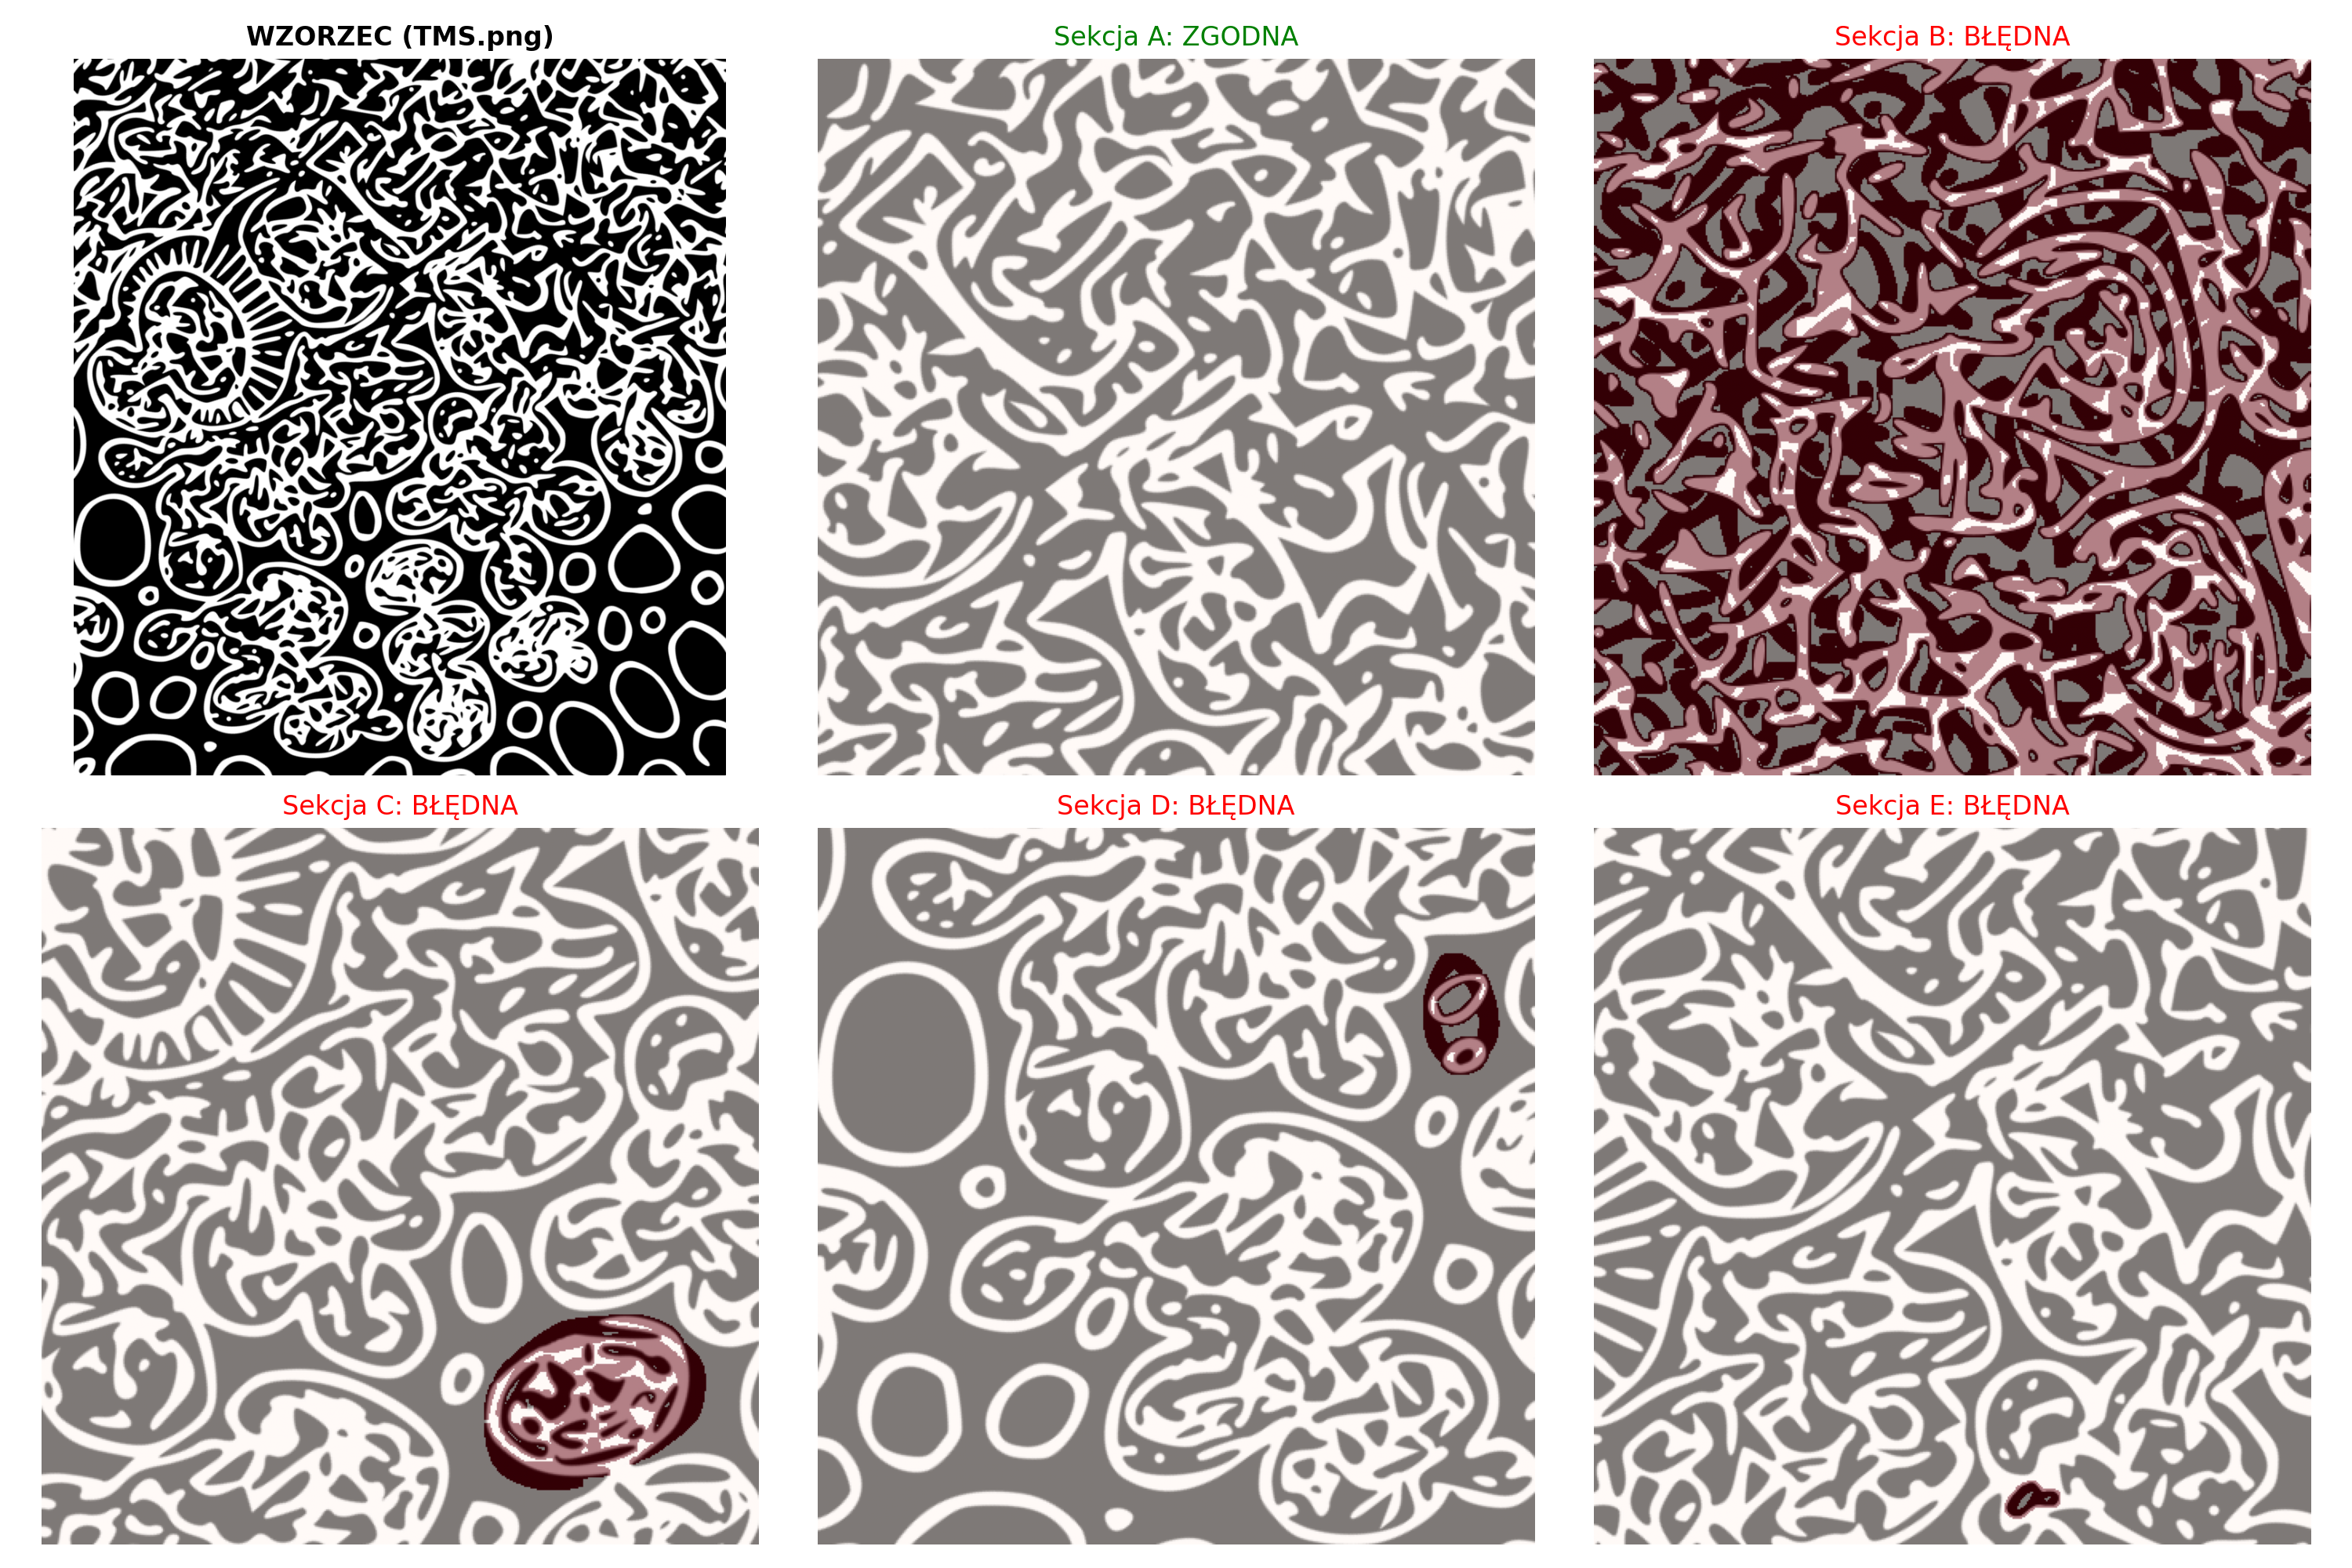
\includegraphics[width=\textwidth]{zad5/Zestawienie_TMS_Wyniki.png}
\caption{Zestawienie: wzorzec \texttt{TMS.png} oraz wynik porównania każdej z sekcji A--E. Czerwone obszary to piksele, w których sekcja różni się od wzorca powyżej progu.}
\end{figure}

\end{document}
